% This work is licensed under the Creative Commons
% Attribution-NonCommercial-ShareAlike 4.0 International License. To view a copy
% of this license, visit http://creativecommons.org/licenses/by-nc-sa/4.0/ or
% send a letter to Creative Commons, PO Box 1866, Mountain View, CA 94042, USA.

\documentclass[12pt,a4paper]{article} 

% This work is licensed under the Creative Commons
% Attribution-NonCommercial-ShareAlike 4.0 International License. To view a copy
% of this license, visit http://creativecommons.org/licenses/by-nc-sa/4.0/ or
% send a letter to Creative Commons, PO Box 1866, Mountain View, CA 94042, USA.

% PACKAGES
\usepackage[english, ngerman]{babel}	% Paket für Sprachselektion, in diesem Fall für deutsches Datum etc
\usepackage[utf8]{inputenc}	% Paket für Umlaute; verwende utf8 Kodierung in TexWorks 
\usepackage[T1]{fontenc} % ö,ü,ä werden richtig kodiert
\usepackage{amsmath} % wichtig für align-Umgebung
\usepackage{amssymb} % wichtig für \mathbb{} usw.
\usepackage{amsthm} % damit kann man eigene Theorem-Umgebungen definieren, proof-Umgebungen, etc.
\usepackage{mathrsfs} % für \mathscr
\usepackage[backref]{hyperref} % Inhaltsverzeichnis und \ref-Befehle werden in der PDF-klickbar
\usepackage{graphicx}
\usepackage{grffile}
\usepackage{setspace} % wichtig für Lesbarkeit. Schöne Zeilenabstände
\usepackage{enumitem} % für custom Liste mit default Buchstaben
\usepackage{ulem} % für bessere Unterstreichung
\usepackage{contour} % für bessere Unterstreichung
\usepackage{epigraph} % für das coole Zitat
\usepackage{float}            % figure-Umgebungen besser positionieren
\usepackage{xfrac}
\usepackage{bbm} %sorgt für Symbol für Indikatorfunktion
\usepackage{color} % bringt Farbe ins Spiel
\usepackage{pdflscape} % damit kann man einzelne Seiten ins Querformat drehen
\usepackage{aligned-overset} % besseres Einrücken, siehe: https://tex.stackexchange.com/questions/257529/overset-and-align-environment-how-to-get-correct-alignment
\usepackage{pgfplots}
	\pgfplotsset{compat=newest}

\usepackage[
    type={CC},
    modifier={by-nc-sa},
    version={4.0},
]{doclicense} % für CC Lizenz-Vermerk

\usepackage{tikz}
  \usetikzlibrary{matrix}
  \usetikzlibrary{cd}
  \usetikzlibrary{babel}
  \usetikzlibrary{calc}
	\usetikzlibrary{positioning}
	\usetikzlibrary{shapes.geometric}
	\usetikzlibrary{fit}
	\usetikzlibrary{arrows}
	
\usepackage{csquotes}
	\MakeOuterQuote{"}

\usepackage{xargs} % for multiple optional args in newcommand
\usepackage{lmodern} % provides a bigger set of font sizes
\usepackage{anyfontsize} % supports fallback scaling for non-existing font size
\usepackage{scrhack} % provides a hack for deprecated float environments used by some libs

% Ich habe gelesen, dass man folgendes Package zuletzt einbinden soll:
\usepackage[english, ngerman, capitalise]{cleveref} % bessere Verweise

% This work is licensed under the Creative Commons
% Attribution-NonCommercial-ShareAlike 4.0 International License. To view a copy
% of this license, visit http://creativecommons.org/licenses/by-nc-sa/4.0/ or
% send a letter to Creative Commons, PO Box 1866, Mountain View, CA 94042, USA.

% THEOREM-ENVIRONMENTS

\newtheoremstyle{mystyle}
  {20pt}   % ABOVESPACE \topsep is default, 20pt looks nice
  {20pt}   % BELOWSPACE \topsep is default, 20pt looks nice
  {\normalfont} % BODYFONT
  {0pt}       % INDENT (empty value is the same as 0pt)
  {\bfseries} % HEADFONT
  {}          % HEADPUNCT (if needed)
  {5pt plus 1pt minus 1pt} % HEADSPACE
	{}          % CUSTOM-HEAD-SPEC
\theoremstyle{mystyle}

% Definitionen der Satz, Lemma... - Umgebungen. Der Zähler von "satz" ist dem "section"-Zähler untergeordnet, alle weiteren Umgebungen bedienen sich des satz-Zählers.
\newtheorem{satz}{Satz}[section]
\newtheorem{lemma}[satz]{Lemma}
\newtheorem{korollar}[satz]{Korollar}
\newtheorem{proposition}[satz]{Proposition}
\newtheorem{beispiel}[satz]{Beispiel}
\newtheorem{definition}[satz]{Definition}
\newtheorem{bemerkungnr}[satz]{Bemerkung}
\newtheorem{theorem}[satz]{Theorem}
\newtheorem{erinnerungnr}[satz]{Erinnerung}
\newtheorem{vermutung}[satz]{Vermutung}

% Bemerkungen, Erinnerungen und Notationshinweise werden ohne Numerierungen dargestellt.
\newtheorem*{bemerkung}{Bemerkung.}
\newtheorem*{erinnerung}{Erinnerung.}
\newtheorem*{notation}{Notation.}
\newtheorem*{aufgabe}{Aufgabe.}
\newtheorem*{lösung}{Lösung.}
\newtheorem*{beisp}{Beispiel.}  %Beispiel ohne Nummerierung
\newtheorem*{defi}{Definition.} %Definition ohne Nummerierung
\newtheorem*{lem}{Lemma.}       %Lemma ohne Nummerierung
\newtheorem*{thm}{Theorem.}     %Theorem ohne Nummerierung
\newtheorem*{konvention}{Konvention.}  


% This work is licensed under the Creative Commons
% Attribution-NonCommercial-ShareAlike 4.0 International License. To view a copy
% of this license, visit http://creativecommons.org/licenses/by-nc-sa/4.0/ or
% send a letter to Creative Commons, PO Box 1866, Mountain View, CA 94042, USA.

% STANDARD SHORTCUTS
%%%%%%%%%%%%%%%%%%%%%%%%%%%%%%%%%%%%%%%%%%%%
\newcommand{\R}{\mathbb{R}}				 % reelle Zahlen
\newcommand{\Rn}{\R^n}					 % der R^n
\newcommand{\N}{\mathbb{N}}				 % natürliche Zahlen
\newcommand{\Q}{\mathbb{Q}}				 % rationale Zahlen
\newcommand{\Z}{\mathbb{Z}}				 % ganze Zahlen
\newcommand{\C}{\mathbb{C}}			   % komplexe Zahlen
\renewcommand{\mit}{\text{ mit }}   % mit
\newcommand{\falls}{\text{falls }} % falls
\renewcommand{\d}{\text{ d}}        % Differential d
\DeclareMathOperator{\tr}{tr} % spur
\DeclareMathOperator{\diag}{diag}
\DeclareMathOperator{\Hom}{Hom}
\DeclareMathOperator{\Span}{span}
\DeclareMathOperator{\im}{im}
\DeclareMathOperator{\SO}{SO}
\newcommand{\ideal}{\trianglelefteq} %Ideal
\newcommand{\properideal}{\mathrel{\ooalign{$\lneqq$\cr\raise.51ex\hbox{$\lhd$}\cr}}} %echtes Ideal
\DeclareMathOperator{\supp}{supp}                 % Träger
\newcommandx{\bracket}[2][1=\cdot, 2=\cdot]{[#1,#2]}
\DeclareMathOperator{\graph}{graph}       % Graph einer Funktion

% ETWAS SPEZIELLERE ZEICHEN
%%%%%%%%%%%%%%%%%%%%%%%%%%%%%%%%%%%%%%%%%%%%
% disjunkte Vereinigung
\newcommand{\bigcupdot}{
	\mathop{\vphantom{\bigcup}\mathpalette\setbigcupdot\cdot}\displaylimits
}
\newcommand{\setbigcupdot}[2]{\ooalign{\hfil$#1\bigcup$\hfil\cr\hfil$#2$\hfil\cr\cr}}
% großes Kreuz
\newcommand*{\bigtimes}{\mathop{\raisebox{-.5ex}{\hbox{\huge{$\times$}}}}} 
% dreifach gestrichene Norm
\newcommand{\Vertiii}[1]{{\left\vert\kern-0.25ex\left\vert\kern-0.25ex\left\vert #1 
    \right\vert\kern-0.25ex\right\vert\kern-0.25ex\right\vert}}
% korrektes argmin und argmax
\DeclareMathOperator*{\argmax}{arg\,max}
\DeclareMathOperator*{\argmin}{arg\,min}

% WHITESPACE COMMANDS
%%%%%%%%%%%%%%%%%%%%%%%%%%%%%%%%%%%%%%%%%%%%
% Zeilenumbruch mit freier Zeile darunter OHNE underfull-hbox-warning
\newcommand{\nl}{\\[\baselineskip]}
% nicht restriktiver newline command
\newcommand{\enter}{$ $\newline} 
% praktischer Tabulator
\newcommand\tab[1][1cm]{\hspace*{#1}}

% TEXT ÜBER ZEICHEN
\newcommand{\stackeq}[1]{\stackrel{#1}{=}} 

% TEXT ÜBER UND UNTER ZEICHEN
\newcommand{\stackrelnew}[3]{\underset{#1}{\overset{#2}{#3}}}

% UNDERLINE (wird nicht mehr genutzt)
% besseres underline 
%\renewcommand{\ULdepth}{1pt}
%\contourlength{0.5pt}
%\newcommand{\ul}[1]{
%	\uline{\phantom{#1}}\llap{\contour{white}{#1}}
%}
\newcommand{\ul}[1]{\underline{#1}} %Umleitung des Commands, da man sich gegen obigen entschieden hat. Dieser erzeugt zu viel Whitespace vor und nach dem Unterstrichenem.

% Commands für Stochastik / Statistik
\newcommand{\A}{\mathcal{A}}
\renewcommand{\P}{\mathbb{P}}
\newcommand{\E}{\mathbb{E}}
\newcommand{\B}{\mathcal{B}} %Borel-Sigma-Algebra
\newcommand{\Var}{\mathbb{V}\text{ar}}
\newcommand{\Cov}{\mathbb{C}\text{ov}} %Kovarianz
\newcommand{\indi}{\mathbbm{1}} % Indikatorfunktion
\renewcommand{\L}{\mathcal{L}} %L_p-Räume

% Verteilungen
\DeclareMathOperator{\Bin}{Bin}       %Binomialverteilung
\newcommand{\Nor}{\mathcal{N}}        %Normalverteilung
\DeclareMathOperator{\Poi}{Poi}       %Poissonverteilung
\DeclareMathOperator{\Exp}{Exp}       %Exponentialverteilung
\DeclareMathOperator{\Cauchy}{Cauchy} %Cauchyverteilung


% This work is licensed under the Creative Commons
% Attribution-NonCommercial-ShareAlike 4.0 International License. To view a copy
% of this license, visit http://creativecommons.org/licenses/by-nc-sa/4.0/ or
% send a letter to Creative Commons, PO Box 1866, Mountain View, CA 94042, USA.

\newcommand{\gdw}{\Leftrightarrow}             % genau dann, wenn


\author{Willi Sontopski}

\parindent0cm %Ist wichtig, um führende Leerzeichen zu entfernen

\usepackage{pdflscape}
\usepackage{rotating}
\usepackage{scrpage2}
\pagestyle{scrheadings}
\clearscrheadfoot

\ihead{Willi Sontopski}
\chead{Formale Systeme WiSe 18 19}
\ohead{}
\ifoot{Blatt 11}
\cfoot{Version: \today}
\ofoot{Seite \pagemark}

\newcommand{\A}{\mathcal{A}}

\begin{document}
%\setcounter{section}{1}

\section*{Aufgabe $\ast$)}
%TODO

\section*{Aufgabe $\ast\ast$)}
%TODO

\section*{Aufgabe 1}
Seien $r,s$ reguläre Ausdrücke, Beachte $r=s:\Longleftrightarrow L(r)=L(s)$ (eigentlich $r\equiv s$). Dann gilt:
\begin{enumerate}[label=\alph*)]
	\item $r+s=s+r$
	\item $(r+s)+t=r+(s+t)$
	\item $(rs)t=r(st)$
	\item $r(s+t)=rs+rt$
	\item $\emptyset^\ast=\varepsilon$
	\item $(r^\ast)^\ast=r^\ast$
	\item $r^\ast=rr^\ast+\varepsilon$
	\item $(\varepsilon+r)^\ast=r^\ast$
\end{enumerate}

\begin{proof}
	\underline{Zeige a):}
	\begin{align*}
		r+s
		\overset{\text{Not}}&=		
		L(r+s)
		\overset{\text{Def}}=
		L(r)\cup L(s)
		\overset{\text{Kommu. von }\cup}=
		L(s)\cup L(r)
		\overset{\text{Def}}=
		L(s+r)
		\overset{\text{Not}}=	
		s+r
	\end{align*}
	\underline{Zeige b):}
	\begin{align*}
		L\big((r+s)+t\big)
		\overset{\text{}}&=
		L(r+s)\cup L(t)\\
		\overset{\text{}}&=
		\big(L(r)\cup L(s)\big)\cup L(t)\\
		\overset{\text{Asso. von }\cup}&=
		L(r)\cup\big(L(s)\cup L(t)\big)\\
		\overset{\text{}}&=
		L(r)\cup L(s+t)\\
		\overset{\text{}}&=
		L\big(r+(s+t)\big)
	\end{align*}
	
	\underline{Zeige c):} "Ersetze Punkt durch Konkatenationsoperator auf Sprachen":
	\begin{align*}
		L\big((r\cdot s)\cdot t\big)
		\overset{\text{}}&=
		L(r\cdot s)\cdot L(t)\\
		\overset{\text{}}&=
		\big(L(r)\cdot L(s)\big)\cdot L(t)\\
		\overset{\text{}}&=
		\big\lbrace ab:a\in L(r)\cdot L(s)\wedge b\in L(t)\big\rbrace\\
		\overset{\text{}}&=
		\Big\lbrace ab:a\in\big\lbrace cd:c\in L(r)\wedge d\in L(s)\big\rbrace\wedge b\in L(t)\Big\rbrace\\
		\overset{\text{}}&=
		\Big\lbrace cdb:\big(c\in L(r)\wedge d\in L(s)\big)\wedge b\in L(t)\Big\rbrace\\
		\overset{\text{Asso. von }\wedge}&=
		\Big\lbrace cdb:c\in L(r)\wedge\big(d\in L(s)\wedge b\in L(t)\big)\Big\rbrace\\
		\overset{\text{}}&=
		\Big\lbrace ce:c\in L(r)\wedge e\in\big\lbrace db:d\in L(s)\wedge b\in L(t)\big\rbrace\Big\rbrace\\
		\overset{\text{}}&=
		\big\lbrace ce:c\in L(r)\wedge e\in L(s)\cdot L(t)\big\rbrace\\
		\overset{\text{}}&=
		L(r)\cdot\big(L(s)\cdot L(t)\big)\\
		\overset{\text{}}&=
		L(r)\cdot L(s\cdot t)\\
		\overset{\text{}}&=
		L\big(r\cdot(s\cdot t)\big)
	\end{align*}
	
	\underline{Zeige d):}
	\begin{align*}
		L\big(r(s+r)\big)
		\overset{\text{Def}}&=
		L(r)\cdot L(s+t)\\
		\overset{\text{}}&=
		L(r)\cdot\big(L(s)\cup L(t)\big)\\
		\overset{\text{Aufgabe 7.2 (a)}}&=
		L(r)\cdot L(s)\cup L(r)\cdot L(t)\\
		\overset{\text{}}&=
		L(r\cdot s)\cup L(r\cdot t)\\
		\overset{\text{}}&=
		L(rs+rt)
	\end{align*}		
	
	\underline{Zeige e):}
	Achtung! Hier ist \underline{nicht} der Kleene-Stern gemeint. 
	Er ist definiert als der Kleene-Stern der Sprache,
	\begin{align*}
		L(\underbrace{\emptyset^\ast}_{\text{Regex}})
		\overset{\text{}}&=
		L(\underbrace{\emptyset}_{\text{Regex}})^\ast
		\overset{\text{}}=
		\underbrace{\emptyset}_{\text{Sprache}}^\ast
		\overset{\text{Def }\ast}=
		\bigcup\limits_{n=0}^\infty
		\overset{\text{}}=
		\varepsilon\cup\emptyset\cup\ldots
		\overset{\text{}}=
		\lbrace\underbrace{\varepsilon}_{\text{leeres W}}\rbrace
		\overset{\text{}}=
		L(\underbrace{\varepsilon}_{\text{Regex}})
	\end{align*}
	
	\underline{Zeige f):}
	\begin{align*}
		L\big((r^\ast)^\ast\big)
		\overset{\text{}}&=
		L(r^\ast)^\ast
		\overset{\text{}}=
		\big(L(r)^\ast\big)^\ast
		\overset{\text{Aufg 7.2 (d)}}=
		L(r)^\ast
		\overset{\text{}}=
		L(r^\ast)
	\end{align*}
	Beachte: Alle $\ast$-Symbole innerhalb $L(\ldots)$ bezeichnen den Sternoperator der regulären Ausdrücke.
	Alle $\ast$-Symbole außerhalb $L(\ldots)$ bezeichnet den Kleene-Stern.
	
	\underline{Zeige g):}
	\begin{align*}
		L(r^\ast)
		\overset{\text{}}&=
		L(r)^\ast\\
		\overset{\text{}}&=
		\bigcup\limits_{n=0}^\infty L(r)^n\\
		\overset{\text{}}&=
		L(r)^0\cup\bigcup\limits_{n=1}^\infty L(r)^n\\
		\overset{\text{}}&=
		L(r)^0\cup L(r)\cdot\left(\bigcup\limits_{n=0}^\infty L(r)^n\right)\\
		\overset{\text{}}&=
		\lbrace\varepsilon\rbrace\cup L(r)\cdot L(r)^\ast\\
		\overset{\text{}}&=
		L(\varepsilon)\cup L(r)\cdot L(r^\ast)\\
		\overset{\text{}}&=
		L(\varepsilon)\cup L(r\cdot r^\ast)\\
		\overset{\text{}}&=
		L(\varepsilon+rr^\ast)\\
		\overset{\text{a)}}&=
		L(rr^\ast+\varepsilon)
	\end{align*}
	
	\underline{Zeige h):}
	\begin{align*}
		L\big((\varepsilon+r)^\ast\big)
		\overset{\text{}}&=
		L(\varepsilon+r)^\ast\\
		\overset{\text{}}&=
		\big(L(\varepsilon)\cup L(r)\big)^\ast\\
		\overset{\text{}}&=
		\big(\lbrace\varepsilon\rbrace\cup L(r)\big)^\ast\\
		\overset{\text{}}&=
		L(r)^\ast\\
		\overset{\text{}}&=
		L(r^\ast)
	\end{align*}
\end{proof}

\section*{Aufgabe 2}
Verwenden Sie die Konstruktion aus dem Beweis von Satz von Kleene (Satz 5.4) und das
Lemma von Arden (Lemma 5.6), um einen regulären Ausdruck $r$ anzugeben, der die von dem
folgenden Automaten $\A$ akzeptierte Sprache repräsentiert (das heißt, es soll $L(r) = L(\A)$ gelten).

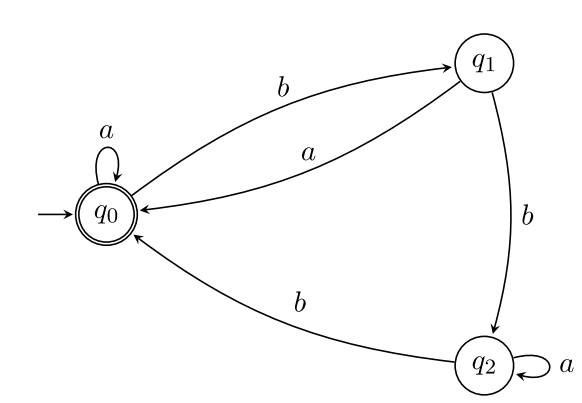
\includegraphics[width=0.7\textwidth]{Blatt11_2.png}
 
\begin{lösung}
	\textbf{Lemma von Arden:}
	Seien $A,B\subseteq\Sigma^\ast$ und $\varepsilon\not\in A$.
	Dann hat
	\begin{align}\label{eqLemmaArden}\tag{Arden}
		X=A\cdot X\cup B
	\end{align}
	die eindeutige Lösung $X=A^\ast\cdot B$.\nl
	Wir erzeugen nun für jeden Zustand $q\in Q$ eine Gleichung.
	\begin{align}\label{eq2_1}
		X_0&=\lbrace a\rbrace\cdot X_0\cup\lbrace b\rbrace\cdot X_1\cdot X_1\cup\lbrace\varepsilon\rbrace\\\label{eq2_2}
		X_1&=\lbrace a\rbrace\cdot X_0\cup\lbrace b\rbrace\cdot X_2\\
		X_2&=\lbrace a\rbrace\cdot X_2\cup\lbrace b\rbrace\cdot X_0\label{eq2_3}
	\end{align}
	Notizen:
	\begin{itemize}
		\item Bei Endzuständen muss $\cup\lbrace\varepsilon\rbrace$ ergänzt werden.
		\item Man schaut sich alle ausgehenden Transitionen an.
	\end{itemize}
	Wende nun Lemma von Arden auf \eqref{eq2_3} an:
	\begin{align}\label{eq2_4}
		X_2&=\lbrace a\rbrace^\ast\cdot\lbrace b\rbrace\cdot X_0 &\text{Lemma auf \eqref{eq2_3}}\\\nonumber
		X_1&=\lbrace a\rbrace\cdot X_0\cup\lbrace b\rbrace\cdot\lbrace a\rbrace^\ast\cdot\lbrace b\rbrace\cdot X_0 &\text{Einsetzen ovon \eqref{eq2_4} in \eqref{eq2_2}}\\
		&=\Big(\lbrace a\rbrace\cup\lbrace b\rbrace\cdot\lbrace a\rbrace^\ast\cdot\lbrace b\rbrace\Big)\cdot X_0\label{eq2_5}\\
		X_0&=\lbrace a\rbrace\cdot X_0\cup\lbrace b\rbrace\Big(\lbrace a\rbrace\cup\lbrace b\rbrace\cdot\lbrace a\rbrace^\ast\cdot\lbrace b\rbrace\Big)\cdot X_0\cup\lbrace\varepsilon\rbrace &\text{Einsetzen von \eqref{eq2_5} in \eqref{eq2_1}}\nonumber\\
		&\overset{\text{Distr}}{=}
		\Big(\lbrace a\rbrace\cup\lbrace b\rbrace\cdot\big(\lbrace a\rbrace\cup\lbrace b\rbrace\cdot\lbrace a\rbrace^\ast\cdot\lbrace b\rbrace\big)\Big)\cdot X_0\cup\lbrace\varepsilon\rbrace\label{eq2_6}\\
		X_0&=\Big(\lbrace a\rbrace\cup\lbrace b\rbrace\cdot\big(\lbrace a\rbrace\cup\lbrace b\rbrace\cdot\lbrace a\rbrace^\ast\cdot\lbrace b\rbrace\big)\Big)^\ast\cdot\lbrace\varepsilon\rbrace &\text{Lemma auf \eqref{eq2_6}}\nonumber\\
		&=L\Big(\big(a+b\cdot(a+ba^\ast b)\big)^\ast\Big)\nonumber\\
		&=L\Big(\big(a+ba+bba^\ast b\big)^\ast\Big)\nonumber
	\end{align}
\end{lösung} 

\section*{Aufgabe 3}
Sei $\Sigma=\lbrace a,b,c\rbrace$. Geben Sie für jede der folgenden Sprachen $L_i$ einen regulären Ausdruck $r_i$ mit $L_i=L(r)$ an.
Erklären Sie die Wahl Ihrer regulären Ausdrücke $r_i$.

\begin{enumerate}[label=\alph*)]
	\item $L_1=\big\lbrace w\in\Sigma^\ast:w\text{ beginnt mit $a$ mit $|w|_b$ ist gerade}\big\rbrace$
	\item $L_2=\big\lbrace w\in\Sigma^\ast:\nexists u,v\in\Sigma^\ast:w=uaav\big\rbrace$
\end{enumerate}

\begin{lösung}
	Idee: 
	\begin{enumerate}
		\item Konstruiere NEA $\A_i$ mit $L(\A_i)=L_i$.
		\item Ermittle den regulären Ausdruck $r_i$ von $\A_i$ wie in Aufgabe 2.
	\end{enumerate}		

	\underline{Zeige a):}
	
	\usetikzlibrary{positioning,automata}
\begin{tikzpicture}[shorten >=1pt,node distance=2.7cm,on grid]
  \node[state,initial]   	(q_0)                		{$q_0$};
  \node[state, accepting] 	(q_1) [above right=of q_0] 	{$q_1$};
  \node[state] 	(q_2) [below=of q_1] 		{$q_2$};
  \path[->] (q_0) edge [bend left=0] node [above] {a} (q_1)
            (q_1) edge [loop right] node [above] {a,c} ()
            	  edge [bend left=30] node [left] {b} (q_2)
            (q_2) edge [loop right] node [right] {a,c} ()
                  edge [bend left=30] node [right] {b} (q_1)
       ;
\end{tikzpicture}

	$q_1\hat{=}$ "gerade Anzahl von b's gelesen"\\
	$q_2\hat{=}$ "ungerade Anzahl von b's gelesen"
	
	\begin{align}
		X_0&=\lbrace a\rbrace\cdot X_1\\
		X_1&=\lbrace a,c\rbrace\cdot X_1\cup\lbrace b\rbrace\cdot X_2\cup\lbrace\varepsilon\rbrace\\
		X_2&=\lbrace a,c\rbrace\cdot X_2\cup\lbrace b\rbrace\cdot X_1
	\end{align}
	
	Mit dem Lemma von Arden erhalten wir (anwenden auf letzte Gleichung):
	\begin{align*}
		X_2&=\lbrace a,c\rbrace^\ast\cdot\lbrace b\rbrace\cdot X_1\\
		X_1&=\lbrace a,c\rbrace\cdot X_1\cup\lbrace b\rbrace\cdot\lbrace a,c\rbrace^\ast\cdot\lbrace b\rbrace\cdot X_1\cup\lbrace\varepsilon\rbrace\\
		&=\Big(\lbrace a,c\rbrace\cup\lbrace b\rbrace\cdot\lbrace a,c\rbrace^\ast\cdot\lbrace b\rbrace\Big)\cdot X_1 \cup\lbrace\varepsilon\rbrace\\
		X_1&=\Big(\lbrace a,c\rbrace\cup\lbrace b\rbrace\cdot\lbrace a,c\rbrace^\ast\cdot\lbrace b\rbrace\Big)^\ast\cdot\lbrace\varepsilon\rbrace\\
		X_0&=\lbrace a\rbrace\cdot\Big(\lbrace a,c\rbrace\cup\lbrace b\rbrace\cdot\lbrace a,c\rbrace^\ast\cdot\lbrace b\rbrace\Big)^\ast\\
		&=L\Big(a\cdot\big((a+c)+b(a+c)^\ast b\big)^\ast\Big)=:r_i
	\end{align*}		
	
	\underline{Zeige b):}
	Sprache umschreiben:
	\begin{align*}
		L_2&=\big\lbrace w\in\Sigma^\ast:\nexists u,v\in\Sigma^\ast:w=uaav\big\rbrace\\
		&=\big\lbrace w\in\Sigma^\ast: w\text{ enthält keine zwei aufeinanderfolgenden $a$'s}\big\rbrace
	\end{align*}
	
	\begin{tikzpicture}[shorten >=1pt,node distance=2.7cm,on grid]
  \node[state,initial, accepting](q_0)           		{$q_0$};
  \node[state, accepting] 	(q_1) [right=of q_0] 	{$q_1$};
  \path[->] (q_0) edge [loop above] node [above] {b,c} ()
  				  edge [bend left=30] node [above] {a} (q_1)
            (q_1) edge [bend left=30] node [below] {b,c} (q_0)
       ;
	\end{tikzpicture}

	\begin{align*}
		r_1=\big(b+c+a\cdot(b+c)\big)^\ast\cdot(a+\varepsilon)
	\end{align*}
	
	
\end{lösung}

\end{document}
